\documentclass[aspectratio=169,t,11pt,table]{beamer}
% xcolor and define colors -------------------------
\usepackage{xcolor}

% https://www.viget.com/articles/color-contrast/
\definecolor{purple}{HTML}{5601A4}
\definecolor{navy}{HTML}{0D3D56}
\definecolor{ruby}{HTML}{9a2515}
\definecolor{alice}{HTML}{107895}
\definecolor{daisy}{HTML}{EBC944}
\definecolor{coral}{HTML}{F26D21}
\definecolor{kelly}{HTML}{829356}
\definecolor{cranberry}{HTML}{E64173}
\definecolor{jet}{HTML}{131516}
\definecolor{asher}{HTML}{555F61}
\definecolor{slate}{HTML}{314F4F}

% Mixtape Sessions
\definecolor{picton-blue}{HTML}{00b7ff}
\definecolor{violet-red}{HTML}{ff3881}
\definecolor{sun}{HTML}{ffaf18}
\definecolor{electric-violet}{HTML}{871EFF}

\newcommand\pictonBlue[1]{{\color{picton-blue}#1}}
\newcommand\sun[1]{{\color{sun}#1}}
\newcommand\electricViolet[1]{{\color{electric-violet}#1}}
\newcommand\violetRed[1]{{\color{violet-red}#1}}

\newcommand\bgPictonBlue[1]{{\colorbox{picton-blue!20!white}{#1}}}
\newcommand\bgSun[1]{{\colorbox{sun!20!white}{#1}}}
\newcommand\bgElectricViolet[1]{{\colorbox{electric-violet!20!white}{#1}}}
\newcommand\bgVioletRed[1]{{\colorbox{violet-red!20!white}{#1}}}

\def\code#1{\texttt{#1}}

% Main theme colors
\definecolor{accent}{HTML}{00b7ff}
\definecolor{accent2}{HTML}{871EFF}
\definecolor{gray100}{HTML}{f3f4f6}
\definecolor{gray800}{HTML}{1F292D}


% Beamer Options -------------------------------------

% Background
\setbeamercolor{background canvas}{bg = white}

% Change text margins
\setbeamersize{text margin left = 15pt, text margin right = 15pt} 

% \alert
\setbeamercolor{alerted text}{fg = accent2}

% Frame title
\setbeamercolor{frametitle}{bg = white, fg = jet}
\setbeamercolor{framesubtitle}{bg = white, fg = accent}
\setbeamerfont{framesubtitle}{size = \small, shape = \itshape}

% Block
\setbeamercolor{block title}{fg = white, bg = accent2}
\setbeamercolor{block body}{fg = gray800, bg = gray100}

% Title page
\setbeamercolor{title}{fg = gray800}
\setbeamercolor{subtitle}{fg = accent}

%% Custom \maketitle and \titlepage
\setbeamertemplate{title page}
{
    %\begin{centering}
        \vspace{20mm}
        {\Large \usebeamerfont{title}\usebeamercolor[fg]{title}\inserttitle}\\
        {\large \itshape \usebeamerfont{subtitle}\usebeamercolor[fg]{subtitle}\insertsubtitle}\\ \vspace{10mm}
        {\insertauthor}\\
        {\color{asher}\small{\insertdate}}\\
    %\end{centering}
}

% Table of Contents
\setbeamercolor{section in toc}{fg = accent!70!jet}
\setbeamercolor{subsection in toc}{fg = jet}

% Button 
\setbeamercolor{button}{bg = accent}

% Remove navigation symbols
\setbeamertemplate{navigation symbols}{}

% Table and Figure captions
\setbeamercolor{caption}{fg=jet!70!white}
\setbeamercolor{caption name}{fg=jet}
\setbeamerfont{caption name}{shape = \itshape}

% Bullet points

%% Fix spacing between items
\let\olditemize=\itemize 
\let\endolditemize=\enditemize 
\renewenvironment{itemize}{\vspace{0.25em}\olditemize \itemsep0.25em}{\endolditemize}

%% Fix left-margins
\settowidth{\leftmargini}{\usebeamertemplate{itemize item}}
\addtolength{\leftmargini}{\labelsep}

%% enumerate item color
\setbeamercolor{enumerate item}{fg = accent}
\setbeamerfont{enumerate item}{size = \small}
\setbeamertemplate{enumerate item}{\insertenumlabel.}

%% itemize
\setbeamercolor{itemize item}{fg = accent!70!white}
\setbeamerfont{itemize item}{size = \small}
\setbeamertemplate{itemize item}[circle]

%% right arrow for subitems
\setbeamercolor{itemize subitem}{fg = accent!60!white}
\setbeamerfont{itemize subitem}{size = \small}
\setbeamertemplate{itemize subitem}{$\rightarrow$}

\setbeamertemplate{itemize subsubitem}[square]
\setbeamercolor{itemize subsubitem}{fg = jet}
\setbeamerfont{itemize subsubitem}{size = \small}








% Links ----------------------------------------------

\usepackage{hyperref}
\hypersetup{
  colorlinks = true,
  linkcolor = accent2,
  filecolor = accent2,
  urlcolor = accent2,
  citecolor = accent2,
}


% Line spacing --------------------------------------
\usepackage{setspace}
\setstretch{1.35}


% \begin{columns} -----------------------------------
\usepackage{multicol}


% Fonts ---------------------------------------------
% Beamer Option to use custom fonts
\usefonttheme{professionalfonts}

% \usepackage[utopia, smallerops, varg]{newtxmath}
% \usepackage{utopia}
\usepackage[sfdefault,light]{roboto}

% Small adjustments to text kerning
\usepackage{microtype}



% Remove annoying over-full box warnings -----------
\vfuzz2pt 
\hfuzz2pt


% Table of Contents with Sections
\setbeamerfont{myTOC}{series=\bfseries, size=\Large}
\AtBeginSection[]{
        \frame{
            \frametitle{Roadmap}
            \tableofcontents[current]   
        }
    }


% Tables -------------------------------------------
% Tables too big
% \begin{adjustbox}{width = 1.2\textwidth, center}
\usepackage{adjustbox}
\usepackage{array}
\usepackage{threeparttable, booktabs, adjustbox}
    
% Fix \input with tables
% \input fails when \\ is at end of external .tex file
\makeatletter
\let\input\@@input
\makeatother

% Tables too narrow
% \begin{tabularx}{\linewidth}{cols}
% col-types: X - center, L - left, R -right
% Relative scale: >{\hsize=.8\hsize}X/L/R
\usepackage{tabularx}
\newcolumntype{L}{>{\raggedright\arraybackslash}X}
\newcolumntype{R}{>{\raggedleft\arraybackslash}X}
\newcolumntype{C}{>{\centering\arraybackslash}X}

% Figures

% \imageframe{img_name} -----------------------------
% from https://github.com/mattjetwell/cousteau
\newcommand{\imageframe}[1]{%
    \begin{frame}[plain]
        \begin{tikzpicture}[remember picture, overlay]
            \node[at = (current page.center), xshift = 0cm] (cover) {%
                \includegraphics[keepaspectratio, width=\paperwidth, height=\paperheight]{#1}
            };
        \end{tikzpicture}
    \end{frame}%
}

% subfigures
\usepackage{subfigure}


% Highlight slide -----------------------------------
% \begin{transitionframe} Text \end{transitionframe}
% from paulgp's beamer tips
\newenvironment{transitionframe}{
    \setbeamercolor{background canvas}{bg=accent!40!black}
    \begin{frame}\color{accent!10!white}\LARGE\centering
}{
    \end{frame}
}


% Table Highlighting --------------------------------
% Create top-left and bottom-right markets in tabular cells with a unique matching id and these commands will outline those cells
\usepackage[beamer,customcolors]{hf-tikz}
\usetikzlibrary{calc}
\usetikzlibrary{fit,shapes.misc}

% To set the hypothesis highlighting boxes red.
\newcommand\marktopleft[1]{%
    \tikz[overlay,remember picture] 
        \node (marker-#1-a) at (0,1.5ex) {};%
}
\newcommand\markbottomright[1]{%
    \tikz[overlay,remember picture] 
        \node (marker-#1-b) at (0,0) {};%
    \tikz[accent!80!jet, ultra thick, overlay, remember picture, inner sep=4pt]
        \node[draw, rectangle, fit=(marker-#1-a.center) (marker-#1-b.center)] {};%
}


% DAGS ----------------------------------------------
\usepackage{tikz}
\usetikzlibrary{shapes,decorations,arrows,calc,arrows.meta,fit,positioning}
% Tikz settings optimized for causal graphs.
\tikzset{
    -Latex,auto,node distance =1 cm and 1 cm,semithick,
    state/.style ={ellipse, draw, minimum width = 0.7 cm},
    point/.style = {circle, draw, inner sep=0.04cm,fill,node contents={}},
    bidirected/.style={Latex-Latex,dashed},
    el/.style = {inner sep=2pt, align=left, sloped}
}


% Beamer tricks -------------------------------------
% Make \pause work in align environments
\makeatletter
\renewrobustcmd{\beamer@@pause}[1][]{%
  \unless\ifmeasuring@%
  \ifblank{#1}%
    {\stepcounter{beamerpauses}}%
    {\setcounter{beamerpauses}{#1}}%
  \onslide<\value{beamerpauses}->\relax%
  \fi%
}
\makeatother

\begin{document}

\imageframe{includes/banner.png}

\begin{frame}{Last Class}
    \vspace{-2.5\baselineskip}
    \begin{minipage}[c][8\baselineskip][c]{\textwidth}
        \begin{align*}
            \hat{\theta} = \argmin_\theta g(\theta) W g(\theta)' \quad\text{where}&\quad g(\theta) = \frac{1}{N} \sum_{t \in \mathcal{T}} \sum_{j \in \mathcal{J}_t} \overbrace{(\delta_{jt} - x_{jt}'\beta)}^{\textstyle\xi_{jt}(\theta)} \cdot z_{jt} \\
            \text{subject to}&\quad s_{jt} = \sum_{i \in \mathcal{I}_t} w_{it} \cdot \frac{\exp[\delta_{jt} + \alt<1>{\mu_{ijt}(\theta)}{x_{jt}'(\Sigma\nu_{it} + \Pi y_{it})}]}{1 + \sum_{k \in \mathcal{J}_t} \exp[\delta_{kt} + \alt<1>{\mu_{ikt}(\theta)}{x_{kt}'(\Sigma\nu_{it} + \Pi y_{it})}]}
        \end{align*}
    \end{minipage}
     \vspace{-0.5\baselineskip}
    \begin{wideitemize}
        \item On day 2, adding preference heterogeneity $\mu_{ijt}$ gave more realistic substitution patterns.
        \pause
        \begin{itemize}
            \item Most common form is $\mu_{ijt} = x_{jt}'(\Sigma\nu_{it} + \Pi y_{it})$ for $\nu_{it} \sim N(0, I)$ and $y_{it}$ from census data.
            \item Implements random coefficients $\beta_{it} \sim N(\beta + \Pi y_{it}, \Sigma\Sigma')$ on characteristics $x_{jt}$ in utility.
        \end{itemize}
        \pause
        \item This required adding consumer type $i$ data to supplement our product $j$ data from day 1.
        \pause
        \item Let's go over your second coding exercise.
    \end{wideitemize}
\end{frame}

\begin{frame}{Limited Cross-Market Variation}
    \begin{wideitemize}
        \item The price cut exercise seems more reasonable with random coefficients.
        \begin{itemize}
            \item Consumers substitute from similar products, particularly along the price dimension.
        \end{itemize}
        \pause
        \item But which random coefficients we can add is limited by variation in our data.
        \begin{itemize}
            \item Recall the linear regression intuition from the last class.
        \end{itemize}
        \pause
        \item Can't credibly estimate a standard deviation in $\Sigma$ on the mushy dummy.
        \begin{itemize}
            \item Same cereals in each market, so no choice set variation along mushy dimension.
            \item Results in unrealistically limited substitution between similar cereals.
        \end{itemize}
        \pause
        \item Also can't estimate a parameter in $\Pi$ on log income alone.
        \begin{itemize}
            \item Market fixed effects are collinear with market-level income means.
            \item Unrealistic that overall cereal preference doesn't vary with income.
        \end{itemize}
    \end{wideitemize}
\end{frame}

\begin{frame}{Within-Market Variation}
    \begin{wideitemize}
        \item Without much cross-market variation, what we really want is within-market variation.
        \pause
        \item ``Micro data'' has information about \alert{individual choices}, not just market-level quantities.
        \pause
        \item Typical example is consumer survey data.
        \begin{itemize}
            \item Internal surveys conducted by firms.
            \item Ad-hoc surveys conducted by academics.
            \item Marketing research datasets (e.g.\ NielsenIQ's Consumer Panel).
            \item Regulatory agencies like the UK's antitrust authority \citep{reynolds2008use}.
        \end{itemize}
    \end{wideitemize}
\end{frame}

\begin{frame}{Intuition for the Running Example}
    \begin{wideitemize}
        \item Imagine surveying people at the supermarket who purchased cereal.
        \pause
        \item \alert{``What was your annual income last year?''}
        \begin{itemize}
            \item Should be informative about a parameter in $\Pi$ on log income alone.
            \item Mean income of cereal purchasers targets how income shifts cereal preference.
        \end{itemize}
        \pause
        \item \alert{``Would you have purchased another mushy cereal if your first choice wasn't available?''}
        \begin{itemize}
            \item Should be informative about a standard deviation in $\Sigma$ on the mushy dummy.
            \item Within-mushy substitution is precisely what we hope this parameter will increase!
        \end{itemize}
        \pause
        \item Let's incorporate answers to these questions into estimation.
        \begin{itemize}
            \item We'll set up a general framework and come back to these when we have notation to do so. 
        \end{itemize}
    \end{wideitemize}
\end{frame}

\section{Micro BLP Estimation}

\begin{frame}{Micro BLP Estimator}
    \vspace{-\baselineskip}
    \begin{minipage}[c][4\baselineskip][c]{\textwidth}
        \begin{equation*}
            \hat{\theta} = \argmin_\theta g(\theta) W g(\theta)' \quad\text{where}\quad g(\theta) =
            \alt<1>{
                \frac{1}{N} \sum_{t \in \mathcal{T}} \sum_{j \in \mathcal{J}_t} (\delta_{jt}(\theta) - x_{jt}'\beta) \cdot z_{jt}
            }{
                \begin{bmatrix}
                    \frac{1}{N} \sum_{j,t} (\delta_{jt}(\theta) - x_{jt}'\beta) \cdot z_{jt} \\
                    \only<2-3>{\alert<2>{\overline{v}_1} - v_1(\theta)}
                    \only<3>{\\ \alert<3>{\overline{v}_2} - v_2(\theta)}
                    \only<4>{\alert<4>{\overline{v}} - v(\theta)}
                    \only<5->{\alert<5>{f(\overline{v})} - f(v(\theta))}
                \end{bmatrix}
            }
        \end{equation*}
    \end{minipage}
    \vspace{-0.5\baselineskip}
    \begin{wideitemize}
        \item We can extend our BLP estimator by matching statistics from consumer surveys.
        \pause
        \begin{enumerate}
            \item \alert<2>{$\overline{v}_1$}: Mean income of cereal purchasers. Matched to the model's prediction $v_1(\theta)$.
            \pause
            \item \alert<3>{$\overline{v}_2$}: Share of cereal purchasers who chose a mushy cereal and would choose another mushy cereal if their first choice wasn't available. Model analogue is $v_2(\theta)$.
        \end{enumerate}
        \pause
        \item Denote the vector of matched statistics by $\alert<4>{\overline{v}} = [\overline{v}_1, \overline{v}_2]'$.
        \pause
        \item Don't have to be averages $\overline{v}$. Can match any smooth function $\alert<5>{f(\overline{v})}$.
        \begin{itemize}
            \item Ratios (e.g.\ mean income given mushy), correlations (e.g.\ between income and price), etc.
        \end{itemize}
        \pause
        \item The resulting ``micro BLP'' estimator is used a lot in industrial organization.
    \end{wideitemize}
\end{frame}

\begin{frame}{Micro BLP Popularity}
    \begin{columns}
        \begin{column}{0.37\textwidth}
            \vspace{-16em}
            \begin{wideitemize}
                \item First popularized by \\ \cite{petrin2002quantifying} and\defcitealias{berry2004differentiated}{BLP (2004)}\citetalias{berry2004differentiated}.
                \visible<2->{\item Used a lot. But each paper has different notation.}
                \visible<3>{\item We'll use the standardized framework for PyBLP from \citet{conlon2023incorporating}.}
            \end{wideitemize}
        \end{column}
         \begin{column}{0.63\textwidth}
            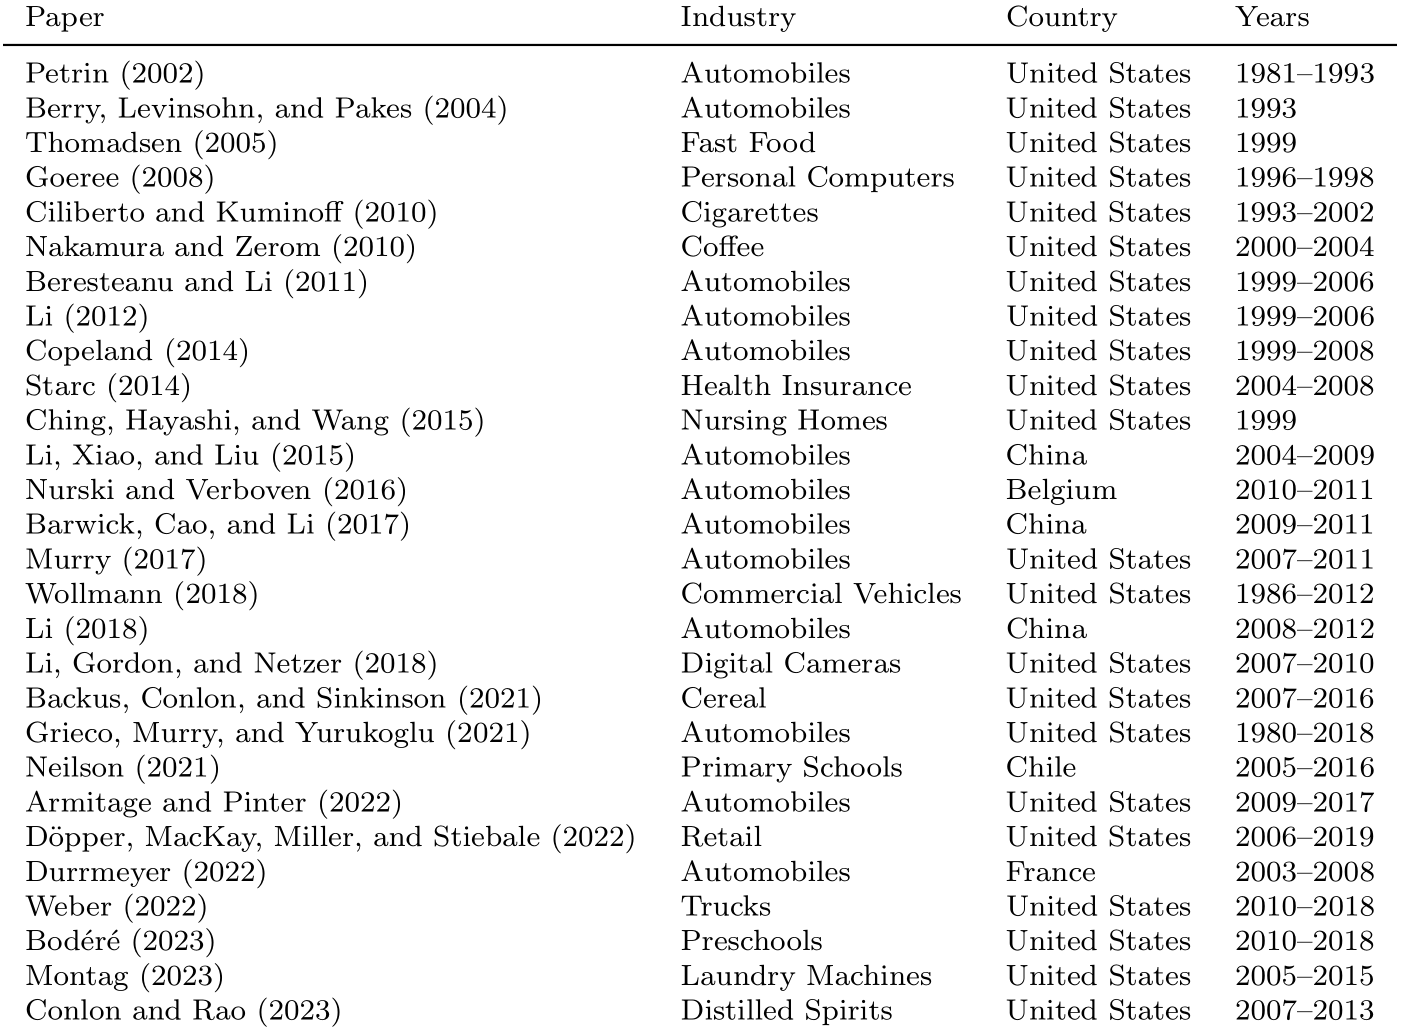
\includegraphics[width=\textwidth]{includes/micro_blp.png}
        \end{column}
    \end{columns}
\end{frame}

\begin{frame}{Micro Moments}
    \begin{equation*}
        \hat{\theta} = \argmin_\theta g(\theta) W g(\theta)' \quad\text{where}\quad g(\theta) =
        \begin{bmatrix}
            \frac{1}{N} \sum_{j,t} (\delta_{jt}(\theta) - x_{jt}'\beta) \cdot z_{jt} \\
            f(\overline{v}) - f(v(\theta))
        \end{bmatrix}
    \end{equation*}
    \begin{wideitemize}
        \item There are two new components.
        \begin{enumerate}
            \item Micro statistics $f(\overline{v}) = [f_1(\overline{v}), \dots, f_M(\overline{v})]'$.
            \item Their model analogues $f(v(\theta)) = [f_1(v(\theta)), \dots, f_M(v(\theta))]'$.
        \end{enumerate}
        \pause
        \item Statistically, we need $f(\overline{v}) \to f(v(\theta_0))$ as the micro dataset expands.
        \begin{itemize}
            \item This gives what we'll call $m = 1, \dots, M$ different ``\alert{micro moments}.''
            \item A bit different from our ``aggregate moments'' $\E[\xi_{jt} \cdot z_{jt}] = 0$.
        \end{itemize}
    \end{wideitemize}
\end{frame}

\begin{frame}{Micro Statistics}
    \begin{wideitemize}
        \item Each micro statistic $f_m(\overline{v})$ is a summary statistic computed on a micro dataset.
        \pause
        \item Micro datasets $d \in \mathcal{D}$ consist of surveyed consumers $n \in \mathcal{N}_d$ who could ...
        \pause
        \begin{enumerate}
            \item ... be from each market $t_n \in \mathcal{T}$ with equal probability.
            \pause
            \item ... be of type $i_n \in \mathcal{I}_{t_n}$ with probability $w_{i_nt_n}$. Same individual type weight as before.
            \pause
            \item ... choose $j_n \in \mathcal{J}_{t_n} \cup \{0\}$ with probability $s_{i_nj_nt_n}$. Same logit choice probability as before.
            \pause
            \item ... be selected into the survey with known probability $w_{di_nj_nt_n}$. Often \alert{choice-based}.
        \end{enumerate}
        \pause
        \item Micro statistics $f_m(\overline{v})$ are smooth functions of $p = 1, \dots, P$ ``micro part'' averages:
        \begin{equation*}
            \overline{v}_p = \frac{1}{N_d} \sum_{n \in \mathcal{N}_d} v_{pi_nj_nt_n}
        \end{equation*}
        \vspace{-\baselineskip}
        \pause
        \item Different weights $w_{dijt}$, values $v_{pijt}$, and functions $f_m(\cdot)$ support most summary stats. 
    \end{wideitemize}
\end{frame}

\begin{frame}{Micro Statistic Example}
    \begin{wideitemize}
        \item To match $\overline{v}_1$, the mean income of cereal purchasers, PyBLP needs some info.
        \pause
        \item First, you need to define your \alert{micro dataset} $d$.
        \begin{itemize}
            \item Sampling weights $w_{dijt} = 1\{j \neq 0\}$ imply only cereal purchasers were surveyed.
            \item In practice, you specify a function to compute a matrix of weights for each market $t$.
            \item You also need to specify the number of survey observations $N_d = |\mathcal{N}_d|$.
        \end{itemize}
        \pause
        \item Second, you need to define your \alert{micro part} $p$.
        \begin{itemize}
            \item Micro values $v_{pijt} = \text{income}_{it}$ means $\overline{v}_p$ is mean surveyed income.
            \item In practice, you specify a second function to compute a matrix of values for each market $t$.
        \end{itemize}
        \pause
        \item Lastly, you need to define your \alert{micro moment} $m$.
        \begin{itemize}
            \item The identity function $f_m(\overline{v}_p) = \overline{v}_p$ just matches the mean surveyed income.
            \item You also need to specify the actual value of the micro statistic $\overline{v}_1$.
        \end{itemize}
    \end{wideitemize}
\end{frame}

\begin{frame}{Model Analogues}
    \vspace{-\baselineskip}
    \begin{minipage}[c][4\baselineskip][c]{\textwidth}
        \begin{equation*}
            f_m\alt<1>{(\overline{v}_p)}{\bigg(\frac{1}{N_d} \sum_{n \in \mathcal{N}_d} v_{pi_nj_nt_n}\bigg)} \to f_m\alt<1>{(v_p(\theta_0))}{\bigg(\frac{\only<2-3>{\cdots} \only<4->{\alert<4>{\sum_{t \in \mathcal{T}}}} \only<4>{\cdots} \only<5->{\alert<5>{\sum_{i \in \mathcal{I}_t}}} \only<6->{\alert<6>{\sum_{j \in \mathcal{J}_t \cup \{0\}}}} \only<5->{\alert<5>{w_{it}}} \only<5>{\cdots} \only<6->{\cdot \alert<6>{s_{ijt}(\theta_0)}} \only<6>{\cdots} \only<7->{\cdot \alert<7>{w_{dijt}} \cdot} \alert<2>{v_{pijt}}}{\only<2-3>{\cdots} \only<4->{\alert<4>{\sum_{t \in \mathcal{T}}}} \only<4>{\cdots} \only<5->{\alert<5>{\sum_{i \in \mathcal{I}_t}}} \only<6->{\alert<6>{\sum_{j \in \mathcal{J}_t \cup \{0\}}}} \only<5->{\alert<5>{w_{it}}} \only<5>{\cdots} \only<6->{\cdot \alert<6>{s_{ijt}(\theta_0)}} \only<6>{\cdots} \only<7->{\cdot \alert<7>{w_{dijt}}}}\bigg)}
        \end{equation*}
    \end{minipage}
     \vspace{-0.5\baselineskip}
    \begin{wideitemize}
        \item For each guess of $\theta$, PyBLP will compute the model analogue $f_m(v_p(\theta))$.
        \pause
        \item The model analogue $v_p(\theta)$ of a micro part $\overline{v}_p$ is a conditional expectation.
        \begin{itemize}
            \item Expected micro value $\alert<2>{v_{pi_nj_nt_n}}$ divided by the probability of being selected.
        \end{itemize}
        \pause
        \item Recall the data generating process for surveyed consumers $n \in \mathcal{N}_d$.
        \pause
        \begin{enumerate}
            \item In market $\alert<4>{t_n \in \mathcal{T}}$ with equal probability.
            \pause
            \item Of type $\alert<5>{i_n \in \mathcal{I}_{t_n}}$ with probability $\alert<5>{w_{i_nt_n}}$.
            \pause
            \item Chooses $\alert<6>{j_n \in \mathcal{J}_{t_n}}$ with probability $\alert<6>{s_{i_nj_nt_n}}$.
            \pause
            \item Selected to be in the survey with known probability $\alert<7>{w_{di_nj_nt_n}}$.
        \end{enumerate}
    \end{wideitemize}
\end{frame}

\section{Choosing Micro Moments}

\begin{frame}{Adding Micro Moments}
    \begin{wideitemize}
        \item Recall my advice from last class about adding instruments.
        \begin{itemize}
            \item For each new parameter, we need another instrument.
            \item Start by choosing a single instrument that ``targets'' that parameter.
        \end{itemize}
        \pause
        \item My advice for adding micro moments is similar.
        \begin{itemize}
            \item For each new parameter without an instrument, we need a micro moment.
            \item Start by choosing a single micro moment that ``targets'' the parameter.
        \end{itemize}
        \pause
        \item What if you could estimate a parameter with either aggregate or micro variation?
        \begin{itemize}
            \item Could just choose the variation that seems more ``credible.'' Often the micro moment.
            \item Can use both. Micro moments can reduce large SEs from limited aggregate variation.
        \end{itemize}
    \end{wideitemize}
\end{frame}

\begin{frame}{Targeting Micro Moments}
    \begin{wideitemize}
        \item Simplest case: 1 characteristic $x_{jt}$ (e.g.\ price), 1 demographic $y_{it}$ (e.g.\ income).
        \begin{equation*}
            u_{ijt} = \alert<4>{\beta_1} + \alert<2>{\pi_1} y_{it} + (\alert<4>{\beta_x} + \alert<3>{\pi_x} y_{it}) x_{jt} + \xi_{jt} + \varepsilon_{ijt} 
        \end{equation*}
        \vspace{-1.5\baselineskip}
        \pause
        \item In our example, matching a ``$\E[y_{it} \mid j \neq 0]$'' micro moment targets \alert<2>{$\pi_1$}.
        \begin{itemize}
            \item Mean income of cereal purchasers targets how income shifts cereal preference.
        \end{itemize}
        \pause
        \item To target \alert<3>{$\pi_x$}, you can match ``$\E[y_{it} \cdot x_{jt} \mid j \neq 0]$'' or similar, e.g.\ ``$\Cov(y_{it}, x_{jt} \mid j \neq 0)$.''
        \begin{itemize}
            \item Relationship between income and price targets how income shifts price sensitivity.
            \item Other common examples include ``$\E[y_{it} \mid x_{jt} < \overline{x}]$'' and ``$\E[x_{jt} \mid y_{it} < \overline{y}]$.''
        \end{itemize}
        \pause
        \item Micro data is not directly informative about ``linear parameters'' \alert<4>{$\beta_1$} or \alert<4>{$\beta_x$}.
        \begin{itemize}
            \item Mean utility $\delta_{jt} = \beta_1 + \beta_x x_{jt} + \xi_{jt}$ is already pinned down by market shares $s_{jt}$.
        \end{itemize}
    \end{wideitemize}
\end{frame}

\begin{frame}{Second Choice Data}
    \begin{wideitemize}
        \item What about targeting unobserved preference heterogeneity parameters in $\Sigma$?
        \pause
        \item The literature has had success with incorporating second choice data\defcitealias{berry2004differentiated}{BLP, 2004}\citepalias[e.g.][]{berry2004differentiated}.
        \begin{itemize}
            \item Survey asks consumers which $k_n \neq j_n$ they'd choose if their first choice weren't available.
            \item Micro weights and values now just have an extra index: $w_{dijkt}$ and $v_{pijkt}$.
        \end{itemize}
        \pause
        \item Direct measures of substitution are very informative about $\Sigma$.
        \begin{itemize}
            \item Recall the red bus/blue bus example that motivated adding preference heterogeneity.
            \item Each second choice is like observing a new market with the first choice removed.
        \end{itemize}
    \end{wideitemize}
\end{frame}

\begin{frame}{Second Choice Moments}
    \begin{wideitemize}
        \item Extend the simple example from before with unobserved preference heterogeneity:
        \begin{equation*}
            u_{ijt} = \beta_1 + \alert<3>{\sigma_1} \nu_{1it} + \pi_1 y_{it} + (\beta_x + \alert<2>{\sigma_x} \nu_{2it} + \pi_x y_{it}) x_{jt} + \xi_{jt} + \varepsilon_{ijt} 
        \end{equation*}
        \vspace{-1.5\baselineskip}
        \pause
        \item To target \alert<2>{$\sigma_x$}, want a measure of how much people substitute within $x_{jt}$.
        \begin{itemize}
            \item In your exercise, you'll match the share ``$\Pr(\text{mushy}_{jt} \text{ and } \text{mushy}_{kt} \mid j \neq 0)$.''
            \item For non-binary $x_{jt}$, can also match ``$\Cov(x_{jt}, x_{kt} \mid j, k \neq 0)$'' or similar.
        \end{itemize}
        \pause
        \item To target \alert<3>{$\sigma_1$}, want a measure of how much people substitute to $k = 0$.
        \begin{itemize}
            \item In your exercise, you'll match another share ``$\Pr(k = 0 \mid j \neq 0)$.''
        \end{itemize}
        \pause
        \item \alert{Diversion ratios} straightforward to interpret and collect.
    \end{wideitemize}
\end{frame}

\begin{frame}{Outside Substitution and Market Size}
    \begin{wideitemize}
        \item Estimating a $\sigma_1$ is important if you're interested in inside-outside substitution.
        \begin{itemize}
            \item How many consumers will stop purchasing soda if all sodas are taxed?
            \item How much larger will a market grow if innovation reduces production costs?
        \end{itemize}
        \pause
        \item On day 1, we discussed how choosing a market size is neither easy nor innocuous.
        \begin{itemize}
            \item Assuming a small market size $M_t$ means assuming a small outside share $s_{0t}$.
            \item Typically, this results in relatively high inside qualities $\xi_{jt}$.
            \item Implies little substitution to the outside good in counterfactuals.
        \end{itemize}
        \pause
        \item Directly matching an outside diversion ratio will help discipline outside substitution.
        \begin{itemize}
            \item If $\hat{\sigma}_1$ is large, many people will dislike all inside goods and usually choose $j = 0$.
            \item This reduces the \textit{effective} market size, helping to compensate for a too-large $M_t$.
            \item See \cite{zhang2023identification} for more on how $\sigma_1$ can help and other solutions.
        \end{itemize}
    \end{wideitemize}
\end{frame}

\section{Using More Information}

\begin{frame}{Information Tradeoffs}
    \begin{wideitemize}
        \item So far we have focused on matching summary statistics. Why not use the full survey?
        \pause
        \item May prefer to use summary stats for a few reasons.
        \pause
        \begin{itemize}
            \item \alert{Cost}: More data costs more. Headline summary stats can be free.
            \pause
            \item \alert{Confidentiality}: Data providers may want to protect respondent identities.
            \pause
            \item \alert{Compatibility}: Aggregate and micro data may come from different sampling schemes.
            \pause
            \item \alert{Clarity}: Matching a single statistic makes it clear where identification comes from.
        \end{itemize}
        \pause
        \item But adding more info can greatly increase the precision of our estimates.
        \begin{itemize}
            \item Ideally we'd observe a complete micro dataset $\{t_n, j_n, k_n, y_{i_nt_n}\}_{n \in \mathcal{N}_d}$.
        \end{itemize}
    \end{wideitemize}
\end{frame}

\begin{frame}{Maximum Likelihood}
    \begin{wideitemize}
        \item If we only had micro data, we may want to just work with its log likelihood: \\
        (technically, this likelihood is conditional on the aggregate data)
        \begin{equation*}
            \log\mathcal{L}(\theta, \delta) = \sum_{n \in \mathcal{N}_d} \log \Pr(t_n, \, j_n, \, k_n, \, y_{i_nt_n} \mid n \in \mathcal{N}_d; \theta, \delta)
        \end{equation*}
        \vspace{-1em}
        \pause
        \item This classic approach proceeds into two steps:
        \pause
        \begin{enumerate}
            \item Find the $\hat{\theta} = (\hat{\Sigma}, \hat{\Pi})$ and mean utilities $\hat{\delta}$ that maximize $\log\mathcal{L}(\theta, \delta)$.
            \pause
            \item Run an IV regression of $\hat{\delta}_{jt}$ on $x_{jt}$ to recover linear parameters $\hat{\beta}$ like in day 1.
        \end{enumerate}
        \pause
        \item For a modern take on this ``MLE'' approach, see \cite*{grieco2022conformant}.
        \begin{itemize}
            \item Combine 1, 2, and the likelihood for aggregate market shares into a single objective.
            \item Their Julia package\defcitealias{grumps}{Grumps.jl}\citetalias{grumps} efficiently handles the high-dimensional $\delta = \{\delta_{jt}\}_{j,t}$.
        \end{itemize}
    \end{wideitemize}
\end{frame}

\begin{frame}{Optimal Micro Moments}
    \begin{wideitemize}
        \item In micro BLP, \alert{optimal micro moments} match the first-order conditions in MLE:
        \begin{equation*}
            f^*(\overline{v}) = \frac{1}{N_d} \sum_{n \in \mathcal{N}_d} \frac{\partial\Pr(t_n, \, j_n, \, k_n, \, y_{i_nt_n} \mid n \in \mathcal{N}_d; \theta)}{\partial\theta}
        \end{equation*}
        \vspace{-\baselineskip}
        \pause
        \item These use all the information in a micro dataset \citep{conlon2023incorporating}.
        \begin{itemize}
            \item Intuition for statistical efficiency here is just that MLE is efficient.
        \end{itemize}
        \pause
        \item Can be a bit tricky to compute, but only a few lines of code with PyBLP.
        \begin{itemize}
            \item Like optimal IVs, can update along with the weighting matrix for a second GMM step.
        \end{itemize}
    \end{wideitemize}
\end{frame}

\section{Coding Exercise 3}

\begin{frame}{Coding Exercise 3}
    \begin{wideitemize}
        \item This is the end of the class, but try to do the third exercise on your own.
        \begin{enumerate}
            \item Incorporating micro moments.
            \item Micro BLP estimation.
            \item Evaluating improvements to the price cut counterfactual.
        \end{enumerate}
        \pause
        \item Also try to the supplemental exercises.
        \begin{itemize}
            \item Varying the market size.
            \item Optimal micro moments.
            \item Estimating a nesting parameter.
        \end{itemize}
        \pause
        \item I'll post the remaining solutions today after questions.
    \end{wideitemize}
\end{frame}

\begin{frame}[c]{}
    \begin{center}
        Good luck with estimating your own demand systems! \\[\baselineskip]
        \href{mailto:jgortmaker@g.harvard.edu}{jgortmaker@g.harvard.edu} \\
        \href{https://twitter.com/jeff_gortmaker}{@jeff\_gortmaker}
    \end{center}
\end{frame}

\backupbegin

\begin{frame}[allowframebreaks,noframenumbering,plain]{References}
    \bibliography{includes/references.bib}
\end{frame}

\backupend

\end{document}